% Slice-wise 2-D reconstruction of a 3-D lightcone (column-width version)
% Build:  cd Figures/src && pdflatex slicewise_reconstruction.tex && mv slicewise_reconstruction.pdf ..
\documentclass[tikz,border=3pt]{standalone}
\usepackage[T1]{fontenc}
\IfFileExists{fourier.sty}{\usepackage{fourier}}{\usepackage{lmodern}}
\usepackage{amsmath,bm}
\usepackage[dvipsnames]{xcolor}
\usetikzlibrary{arrows.meta,positioning,calc,decorations.pathreplacing}

\colorlet{lift}{Gray!18}
\colorlet{gate}{ForestGreen!16}
\colorlet{gateline}{ForestGreen!75!black}
\colorlet{band}{NavyBlue!30}
\colorlet{bandline}{NavyBlue!75!black}

\begin{document}
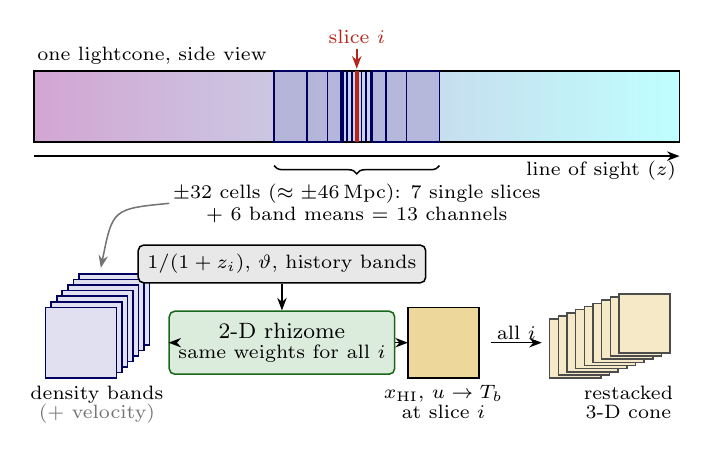
\begin{tikzpicture}[
    font=\footnotesize,
    >={Stealth[length=1.6mm]},
    every path/.style={line width=0.55pt},
    lab/.style={font=\scriptsize, inner sep=1pt},
    blk/.style={draw, rounded corners=2pt, minimum height=0.8cm, minimum width=1.0cm, align=center},
  ]
  % ---------------- lightcone, side view -------------------------------
  \def\cx{4.1}
  \def\hh{0.9}
  \shade[left color=Purple!35, right color=Cyan!25, draw=black] (0,0) rectangle (8.2,\hh);
  \node[lab, anchor=south west] at (0,\hh+0.04) {one lightcone, side view};
  \foreach \a/\b in {0.2/0.37, 0.37/0.63, 0.63/1.05}{
    \fill[band, opacity=0.85] (\cx+\a,0) rectangle (\cx+\b,\hh);
    \draw[bandline] (\cx+\a,0) rectangle (\cx+\b,\hh);
    \fill[band, opacity=0.85] (\cx-\b,0) rectangle (\cx-\a,\hh);
    \draw[bandline] (\cx-\b,0) rectangle (\cx-\a,\hh);
  }
  \foreach \k in {-3,...,3}{
    \draw[bandline, line width=0.7pt] (\cx+0.06*\k,0) -- (\cx+0.06*\k,\hh);
  }
  \draw[BrickRed, line width=1.3pt] (\cx,0) -- (\cx,\hh);
  \node[lab, text=BrickRed, above] at (\cx,\hh+0.3) {slice $i$};
  \draw[BrickRed, ->] (\cx,\hh+0.28) -- (\cx,\hh+0.03);
  \draw[->] (0,-0.18) -- (8.2,-0.18);
  \node[lab, anchor=north east] at (8.2,-0.2) {line of sight ($z$)};
  \draw[decorate, decoration={brace, amplitude=3pt, mirror}] (\cx-1.05,-0.3) -- (\cx+1.05,-0.3);
  \node[lab, align=center] (bl) at (\cx,-0.78) {$\pm32$ cells ($\approx\pm46$\,Mpc): 7 single slices\\ + 6 band means $=$ 13 channels};

  % ---------------- per-slice prediction -------------------------------
  \def\yb{-2.55}
  \foreach \k in {6,...,0}{
    \draw[fill=band!40, draw=bandline] (0.15+0.07*\k,\yb-0.45+0.07*\k) rectangle ++(0.9,0.9);
  }
  \node[lab, align=center, below] at (0.8,\yb-0.5) {density bands\\[-1pt]\textcolor{black!55}{(+ velocity)}};
  \draw[->, black!55] (bl.west) .. controls (1.0,-0.85) .. (0.85,\yb+0.95);

  \node[blk, fill=gate, draw=gateline, minimum width=2.0cm] (R) at (3.15,\yb) {2-D rhizome\\[-2pt]\scriptsize same weights for all $i$};
  \node[blk, fill=lift, font=\scriptsize, minimum height=0.45cm, minimum width=1.0cm] (sc) at (3.15,\yb+1.0) {$1/(1+z_i)$, $\vartheta$, history bands};
  \draw[->] (sc) -- (R);
  \draw[->] (1.75,\yb) -- (R.west);

  \draw[fill=Goldenrod!45, draw=black] (4.75,\yb-0.45) rectangle ++(0.9,0.9);
  \node[lab, align=center, below] at (5.2,\yb-0.5) {$x_{\mathrm{HI}}$, $u\to T_b$\\[-1pt] at slice $i$};
  \draw[->] (R.east) -- (4.75,\yb);

  \draw[->] (5.8,\yb) -- node[lab, above] {all $i$} (6.45,\yb);
  \begin{scope}[shift={(6.55,\yb-0.45)}]
    \foreach \k in {0,...,8}{
      \draw[fill=Goldenrod!25, draw=black!70] (0.11*\k,0.04*\k) rectangle ++(0.65,0.75);
    }
  \end{scope}
  \node[lab, align=center, below] at (7.55,\yb-0.5) {restacked\\[-1pt] 3-D cone};
\end{tikzpicture}
\end{document}
